\documentclass[a4paper,11pt,notitlepage]{article}
\usepackage[utf8]{inputenc}
\usepackage[finnish]{babel}
\usepackage{appendix}
\usepackage{graphicx}
\usepackage{hyperref}
\usepackage{booktabs}
\usepackage[labelfont=bf,labelsep=period]{caption}
\usepackage[style=chem-acs,articletitle=true,maxbibnames=6]{biblatex}
\addbibresource{biblio.bib}
\hyphenation{do-mee-neis-ta sek-vens-sien}

\title{\textit{\normalsize MOLE-211 Bioinformatiikka 1: Harjoitustyö}\\ \textbf{MYO7A}}
\author{Kristian Ojala 017226165}
\date{}

\begin{document}
\maketitle

\renewcommand{\abstractname}{Tiivistelmä}
\begin{abstract}
\textit{MYO7A} on geeni, jonka toiminta on edellytys normaalille näölle, kuulolle ja tasapainoaistille. Sen tuote on moottoriproteiini, jota tarvitaan solun sisäisessä kuljetuksessa. Sitä esiintyy erityisesti värekarvojen yhteydessä. Tässä työssä toteutettiin \textit{MYO7A}:lle yhden geenin fylogeneettinen analyysi.
\end{abstract}

\section{Johdanto}
Myosiini VIIa on epätyypillisiin myosiineihin kuuluva ATP-riippuvainen aktiinia sitova moottoriproteiini, jota koodaa \textit{MYO7A}-geeni. Sitä ilmennetään verkkokalvon pigmenttiepiteelissä, valoreseptorisoluissa, kuuloaistin karvasoluissa sekä tietyissä kiveksen, keuhkon ja munuaisen soluissa \cite{hasson1995,liu1997}. On osoitettu, että MYO7A:ta tarvitaan muun muassa opsiinin kuljetuksessa valoreseptorin yhdysvärekarvan läpi \cite{liu1999}, näkösykliin osallisen RPE65-entsyymin kuljetuksessa \cite{lopes2011} ja spermatidien kuljetuksessa siemenepiteelissä \cite{wen2019}. Mutaatiot \textit{MYO7A}:ssa voivat aiheuttaa peittyvästi autosomissa periytyvän tyypin 1B Usherin oireyhtymän (USH1B) tai sensorineuraalisen huonokuuloisuuden, joka voi periytyä vallitsevasti (DFNA11) tai peittyvästi (DFNB2) \cite{riazuddin2008}. USH1B ilmenee varhaisessa iässä vaikeana tai erittäin vaikeana kuulovikana, verkkokalvon pigmenttirappeumana ja tasapainoelimen toimintahäiriönä.

Tässä työssä tutkittiin, mitä tietoa biotietokannat tarjoavat \textit{MYO7A}:sta ja sen rooleista organelliliikenteessä, sekä selvitettiin geenin evolutiivista konservaatiota 11 eläinlajin välillä.

\section{Menetelmät}
Tiedonhaun ja analyysin kaikki askeleet tehtiin Python-ohjelmointikielellä Jupyter-muistioon, joka on saatavilla osoitteessa \url{https://github.com/ogkristi/bioinfo1}.

Ihmisen MYO7A:sta etsittiin tietoa UniProtKB:sta käyttäen UniProtin verkkosivun REST API:a (https://rest.uniprot.org/uniprotkb/). Geenin Gene Ontology (GO) annotaatioita haettiin UniProt ID:n perusteella QuickGO:n REST API:n (https://www.ebi.ac.uk/QuickGO/services/) kautta. Löytyneistä GO-luokista valittiin satunnaisesti viisi ja niiden esivanhemmista muodostettu graafi noudettiin saman APIn kautta.

Ihmisen \textit{MYO7A} mRNA-sekvenssejä etsittiin Biopythonin \cite{biopython} Entrez-moduulilla NCBI:n RefSeq-tietokannasta. Tuloksista valittiin ensimmäinen (NM\_001127180) analyysiin. Sekvenssille etsittiin mRNA-homologeja kym\-menestä muusta lajista: kapusiiniapina, aasiannorsu, isoviiksisiippa, kaljurotta, kotihiiri, japaninviiriäinen, vuokkokala, sokkeloviuhkapyrstö, kirjokilpikonna ja merisiili (tieteelliset nimet taulukossa \ref{blast}). Haku tehtiin Biopythonin Blast-moduulilla käyttäen blastn-ohjelmaa ja rajaten haku refseq\_rna-tieto\-kantaan. Tuloksista valittiin jokaiselle lajille paras osuma ja niitä vastaavat sekvenssit noudettiin Biopythonin Entrez-moduulilla. Lajivalintoja joutui iteroimaan, sillä esimerkiksi grönlanninhaille ei löytynyt RefSeq:istä mRNA-sekvenssejä ja savanninorsulle paras osuma edusti \textit{MYO7B}:tä.

Sekvenssit rinnastettiin MAFFT v.7.520 \cite{mafftv7} ohjelmiston iteratiivisella L-INS-i algoritmilla käyttäen oletusasetuksia. Rinnastuksen visualisointiin käytettiin Python-pakettia nimeltä pyMSAviz. Sitten usean sekvenssin rinnastuksesta muodostettiin fylogeneettinen puu suurimman uskottavuuden menetelmään perustuvalla IQ-TREE v.2.2.6 \cite{iqtree} ohjelmistolla käyttäen 1000 bootstrap-toistoa ja määräten merisiili ulkoryhmäksi. Puu visualisoitiin Biopythonin Phylo-moduulilla \cite{phylo}.


\section{Tulokset}
\textbf{UniProtKB.} MYO7A kuuluu TRAFAC luokan myosiini-kinesiini ATPaasi superperheeseen ja edelleen myosiinien perheeseen. Proteiini koostuu domeeneista myosiinimoottori, IQ 1-5, MyTH4 1, FERM 1, SH3, MyTH4 2 ja FERM 2. UniProtKB tunnustaa proteiinille 8 vaihtoehtoisen silmukoinnin tuotetta eli isoformia, mutta kommentoi, että isoformeja lienee todellisuudessa enemmän. Proteiinissa on fosforyloitavia seriini- ja treoniinitähteitä.

MYO7A osallistuu solunsisäiseen liikenteeseen sitoutumalla häntäosallaan kalvomaisiin osastoihin ja liikuttamalla niitä aktiinifilamentteja pitkin. Sillä on tärkeitä tehtäviä verkkokalvossa: valoreseptorissa se osallistuu kalvolevyjen uudistamiseen ja opsiinin kuljetuksen sääntelyyn. Pigmenttiepiteelissä se osallistuu melanosomien ja fagosomien sijoitteluun. Sisäkorvassa sillä on tärkeitä tehtäviä karvasolukimppujen erilaistumisessa, morfogeneesissä ja järjestäytymisessä. Se osallistuu karvasoluissa ototoksisten aminoglykosidien kalvorakkulavälitteiseen liikennöintiin. MYO7A, USH1C, USH1G ja CDH23 muodostavat yhdessä verkoston, joka välittää mekanotransduktiota karvasoluissa. MYO7A on välttämätön normaalille kuulolle.

\textbf{QuickGO.} \textit{MYO7A}:lle löytyi 59 ainutlaatuista GO-luokkaa. Molekylaariseen funktioon liittyvät luokat kertovat sen sitovan seuraavia molekyylejä: ATP, ADP, kalmoduliini, aktiini ja spektriini. Solun komponentteja, joihin se voi sijoittua, ovat sukakarva, mikrovillus, melanosomi, valoreseptorin ulompi ja sisempi jaoke sekä yhdysvärekarva, synapsi, solun korteksi ja lysosomin kalvo. Esimerkkejä biologisista prosesseista, joihin se osallistuu, ovat solunsisäinen proteiinien kuljetus, pigmenttijyväsen kuljetus, fagolysosomien kokoonpano, aktiinisäikeiden järjestäytyminen, näkeminen, kuuleminen ja tasapainoaisti. Lisäksi biologisissa prosesseissa tulee esiin korvan ja silmän aistinsolujen erilaistuminen ja morfogeneesi. Viiden GO-luokan esivanhemmista muodostettu graafi on liitekuvassa \ref{gograafi}.

\textbf{Fylogenia.} Taulukossa \ref{blast} on BLAST-osumista analyysiin valittujen sekvenssien tunnisteet ja pituudet. Kaikkien osumien E-arvo oli käytännössä 0. Sekvenssien rinnastuksesta on 800 emäksen pala aloituskodonin ympäristöstä visualisoituna liitekuvassa \ref{msa}. Usean sekvenssin rinnastuksesta muodostettu puu on kuvassa \ref{puu}.

\begin{table}[!h]
	\centering
	\caption{Analyysiin valitut sekvenssit.} \label{blast}
	\begin{tabular}{llrc}
	\toprule
	\textbf{Organismi} & \textbf{Accession} & \textbf{Pituus} \\
	\midrule
	\textit{Homo sapiens} & NM\_001127180 & 7363 \\
	\textit{Cebus imitator} & XM\_017533058 & 7372 \\
	\textit{Elephas maximus} & XM\_049889739 & 9832 \\
	\textit{Myotis brandtii} & XM\_005867033 & 9427 \\
	\textit{Heterocephalus glaber} & XM\_013067417 & 7318 \\
	\textit{Mus musculus} & NM\_008663 & 7361 \\
	\textit{Coturnix japonica} & XM\_015852500 & 7484 \\
	\textit{Amphiprion ocellaris} & XM\_055012531 & 7688 \\
	\textit{Nothobranchius furzeri} & XM\_054734303 & 12445 \\
	\textit{Chrysemys picta} & XM\_042849556 & 8349 \\
	\textit{Lytechinus variegatus} & XM\_041626427 & 7119 \\
	\bottomrule
	\end{tabular}
\end{table}

\begin{figure}[!h]
	\centering
	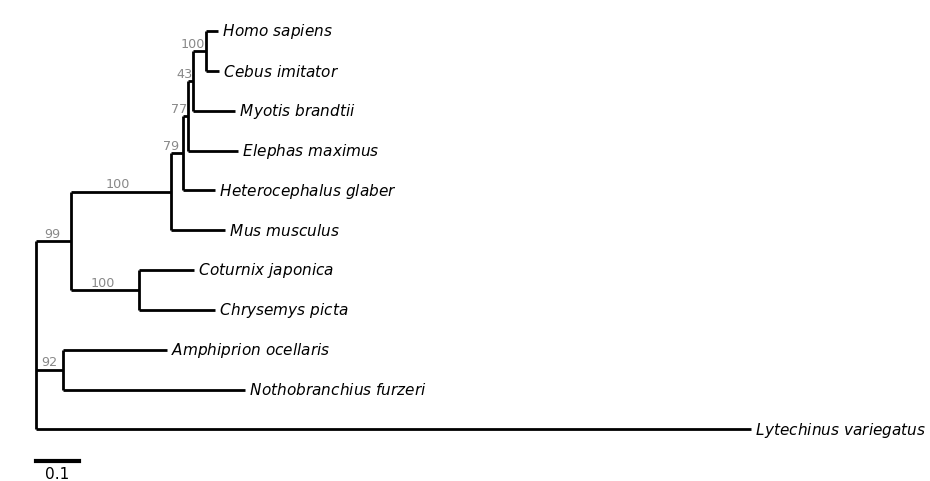
\includegraphics[width=\textwidth]{tree.png}
	\caption{IQ-TREE:n tuottama suurimman uskottavuuden puu. Haarojen bootstrap-tukiarvot ovat harmaita. Oksan pituus merkitsee odotettua emässubstituutioiden lukumäärää per sijainti.} \label{puu}
\end{figure}

\section{Tulosten tarkastelu}
Valtaosa analyysiin hyväksytyistä mRNA-sekvensseistä on ennustuksia, koska harvalle lajille löytyi todellisten transkriptien sekvenssejä. Sekvenssien pituuksissa on jonkun verran hajontaa; ääripäässä \textit{N. furzeri}n sekvenssi on noin viisi tuhatta emästä pidempi kuin ihmisen. MAFFT L-INS-i käyttää sisäisesti paikallista rinnastusta ja dokumentaation mukaan se suoriutuu hyvin, vaikka sekvensseissä olisi huonosti rinnastuvia terminaalisia osuuksia. Rinnastuksen visualisoinnista (kuva \ref{msa}) voi nähdä, että rinnastus on järjellinen aloituskodonista eteenpäin.

Fylogeneettisessä puussa kalat (\textit{A. ocellaris} ja \textit{N. furzeri}), nisäkkäät sekä lintu ja kilpikonna yhdessä (\textit{C. japonica} ja \textit{C. picta}) muodostavat korkealla luottamuksella kukin omat kladinsa. Luottamus on korkea myös kädellisten omaan kladiin (\textit{H. sapiens} ja \textit{C. imitator}). Sen sijaan nisäkkäiden alipuun sisäinen haarautumisjärjestys on epävarma, mihin voi vaikuttaa esimerkiksi se, että kaljurotan ja lepakoiden aistit ovat hyvin erikoistuneet. Puussa ihminen ja kapusiini ovat lähimmät sukulaiset. Lintu ja kilpikonna ovat melko kaukaisia sukulaisia samaan kladiin sijoittumisesta huolimatta. Merisiili (\textit{L. variegatus}) on selvästi kaukaisinta sukua kaikille muille.

Geeni on selvästi alkuperältään todella vanha, sillä sille löytyi ortologi merisiilestä, jolla ei ole varsinaisia silmiä tai korvia. Puun topologiassa saattaa näkyä eläimien aistielimien erilaiset adaptaatiot.

\pagebreak
\printbibliography[title={Kirjallisuusluettelo}]

\pagebreak
\renewcommand{\thefigure}{A\arabic{figure}}
\setcounter{figure}{0}
\begin{appendices}
\renewcommand\thefigure{\thesection.\arabic{figure}} 
\section{Liitteet}

\begin{figure}[!h]
	\centering
	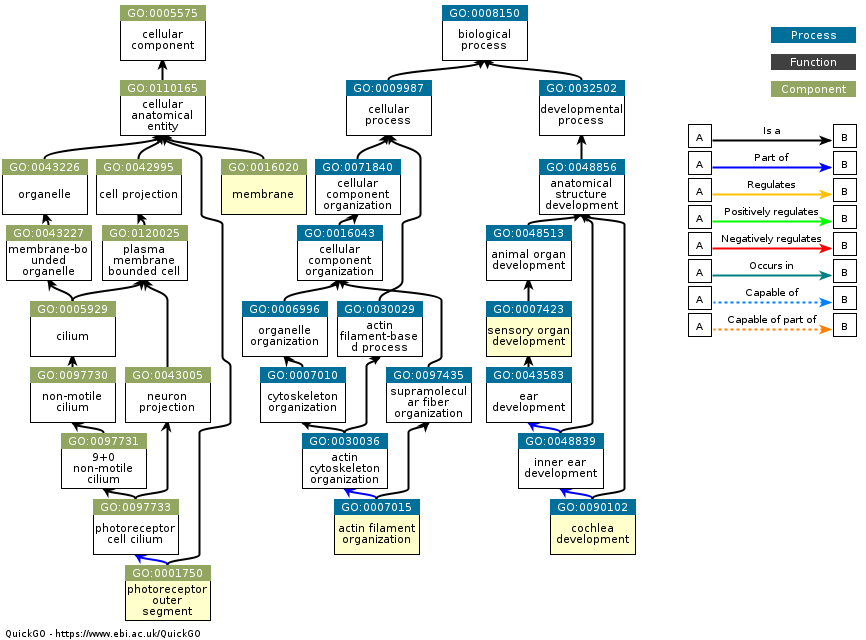
\includegraphics[width=\textwidth]{gochart.png}
	\caption{GO-graafi.} \label{gograafi}
\end{figure}

\pagebreak
\begin{figure}[!h]
	\centering
	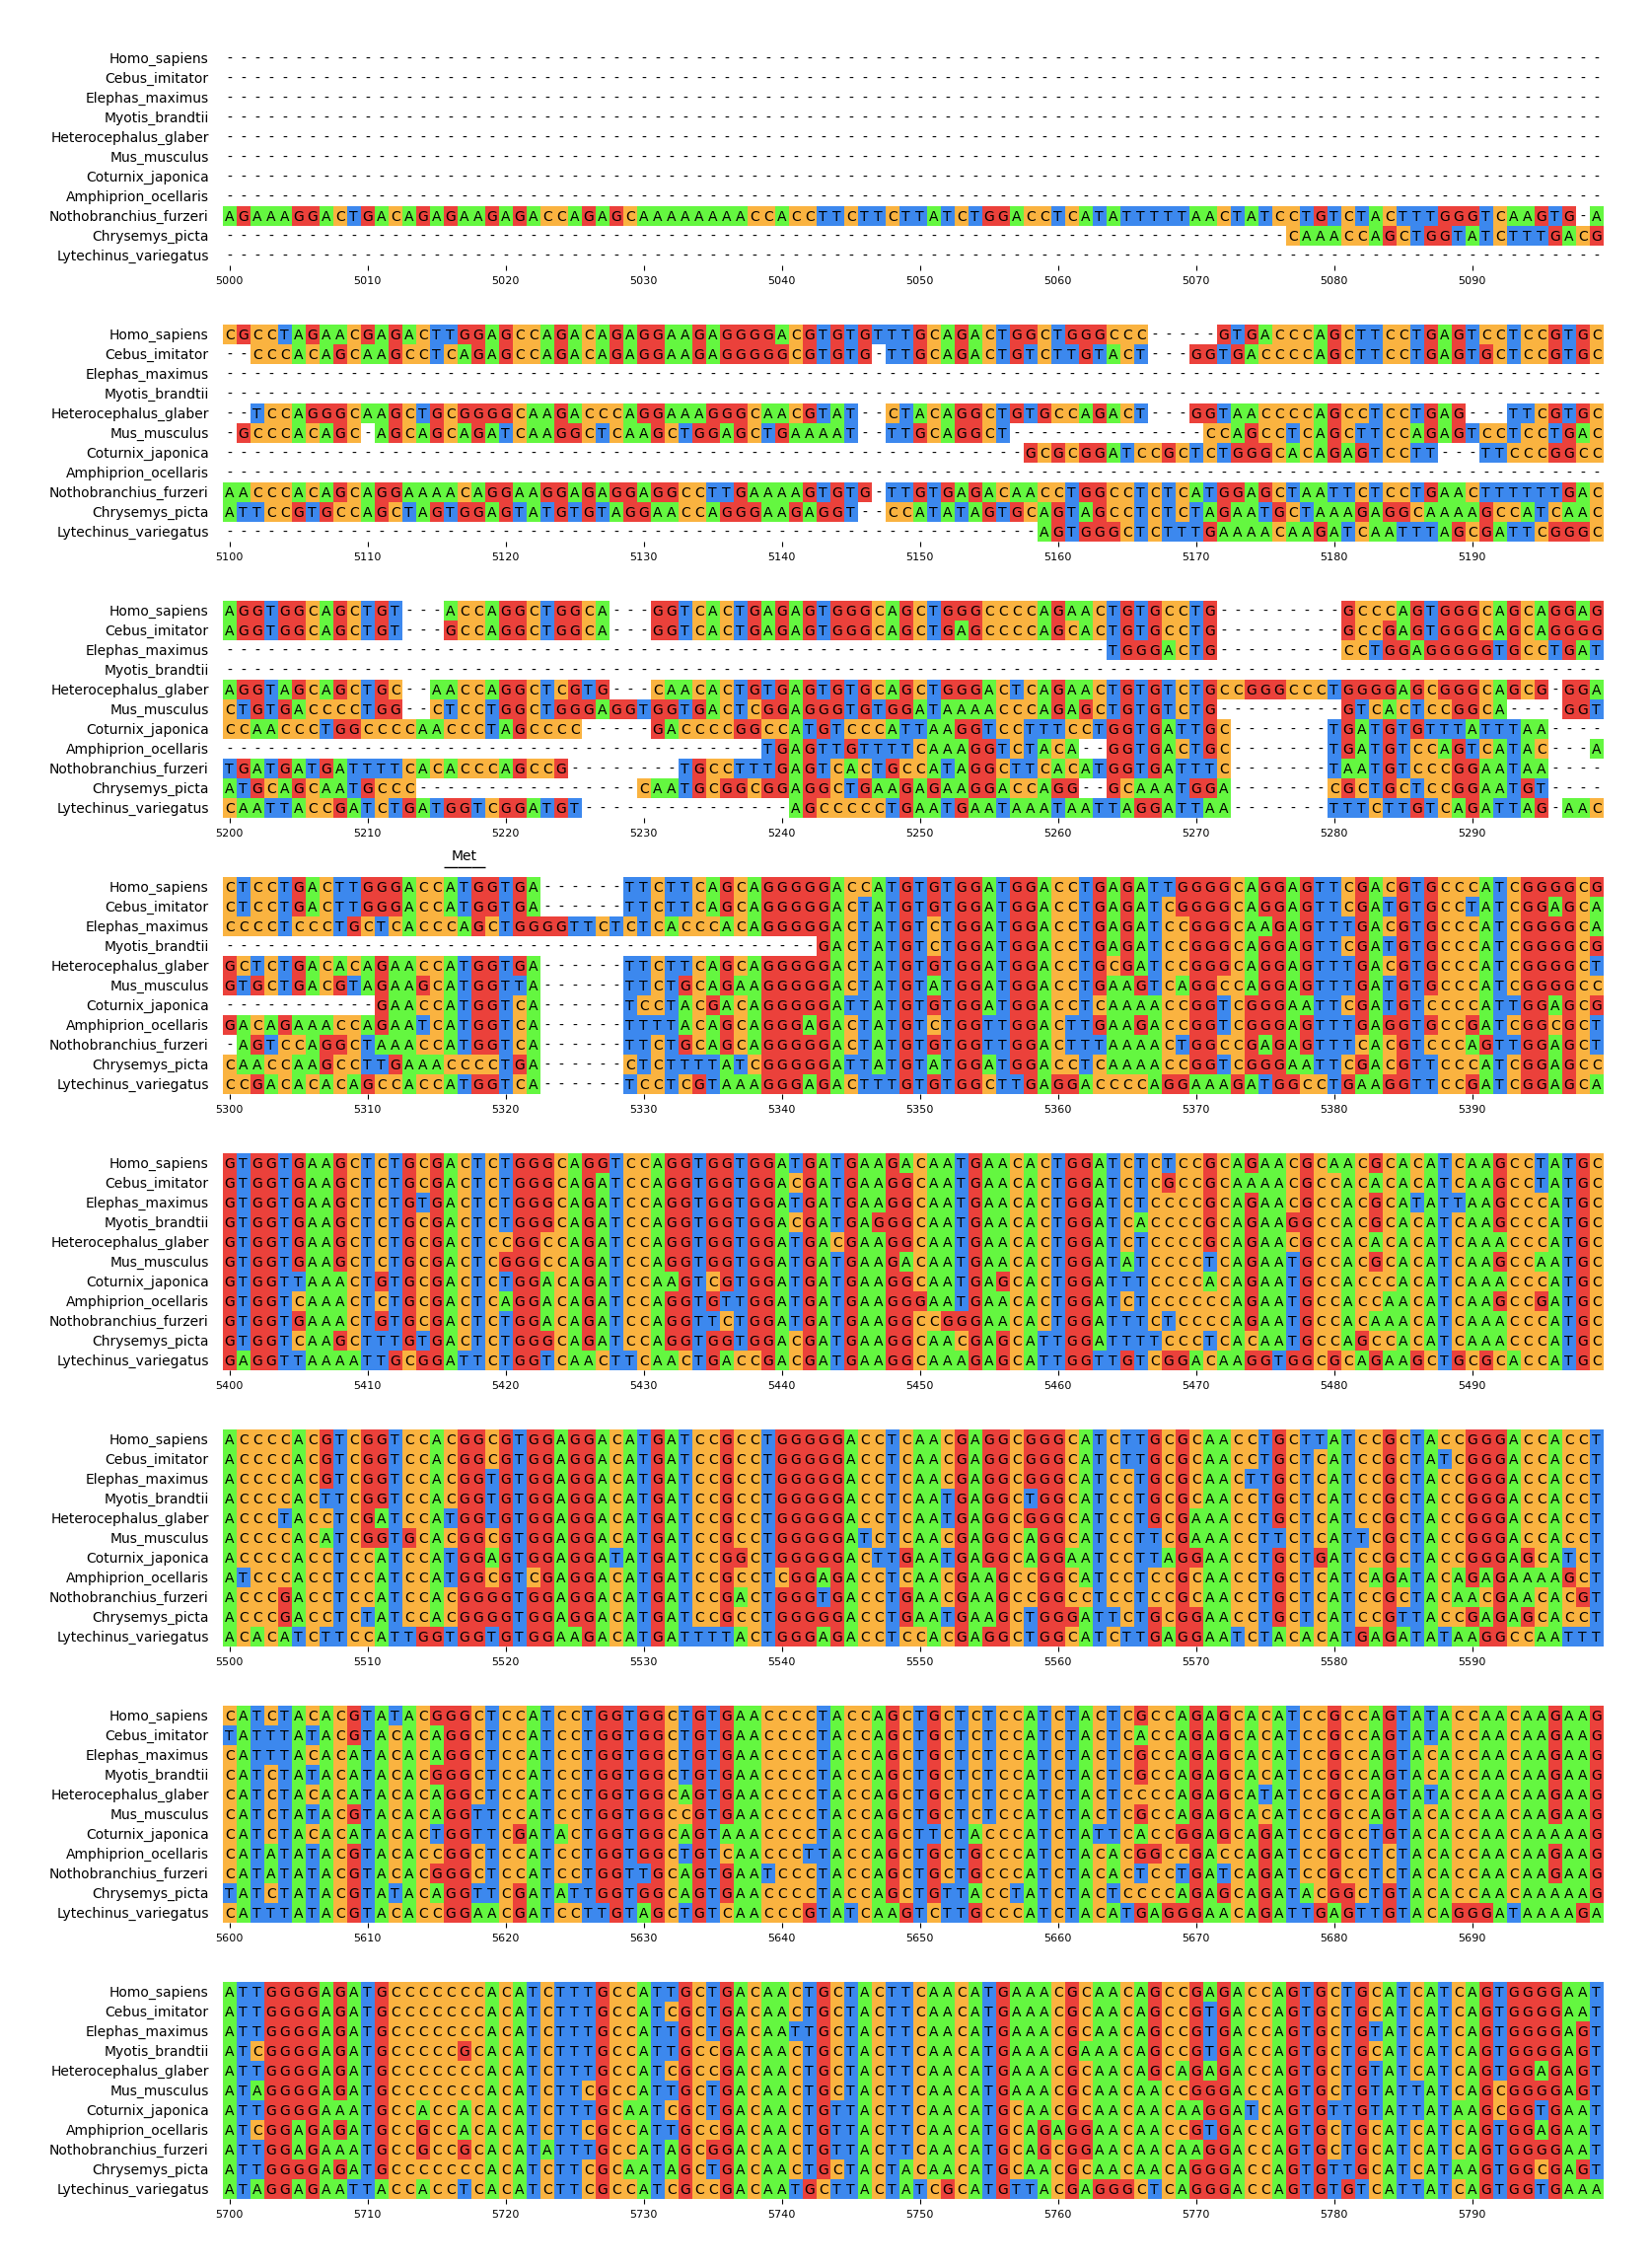
\includegraphics[width=\textwidth]{msa.png}
	\caption{Osa usean sekvenssin rinnastuksesta. Ihmisen aloitusmetioniini on merkattuna kohdassa 5316.} \label{msa}
\end{figure}

\end{appendices}

\end{document}